\documentclass[a4paper,14pt]{extarticle} \usepackage[utf8]{inputenc}
\usepackage[T1]{fontenc}
\usepackage[margin=2.5cm]{geometry}

% Fonte Caladea se existir, senão lmodern
\IfFileExists{caladea.sty}{
  \usepackage{caladea}
}{
  \usepackage{lmodern} }
\usepackage{ragged2e}
\usepackage{graphicx}
\usepackage[portuguese]{babel}
\usepackage{wrapfig}
\usepackage{hyperref}
\usepackage{fancyhdr}
\usepackage{xcolor}
\usepackage{rotating}
\usepackage{titlesec}
\usepackage{epigraph}
\usepackage{dirtytalk}
\usepackage{indentfirst} % Indenta o primeiro parágrafo após seções

% Ajuste do recuo de parágrafo
\setlength{\parindent}{1.5em}

% Adjust headheight to remove LaTeX warning
\setlength{\headheight}{17.54163pt}

% Centralizar títulos
\titleformat{\section}
  {\normalfont\centering\bfseries\Large}{}{1em}{}

\titleformat{\subsection}
  {\normalfont\centering\bfseries\large}{}{1em}{}

\titleformat{\subsubsection}
  {\normalfont\centering\bfseries}{}{1em}{}

% -------------- Símbolos de Versículo e Resposta --------------
% Definição do símbolo (a “barrinha” inclinada)
\makeatletter
\newcommand{\vers@resp@sym}{%
  \raisebox{0.2ex}{\rotatebox[origin=c]{-20}{$\m@th\rceil$}}%
}
% macro interna que sobrepõe a barrinha e a letra V ou R
\newcommand{\vers@resp}[2]{%
  {\ooalign{%
     \hidewidth\kern#1\vers@resp@sym\hidewidth\cr
     #2\cr
  }}%
}
% comandos públicos \versicle e \response
\DeclareRobustCommand{\versicle}{\vers@resp{-0.1em}{V}}
\DeclareRobustCommand{\response}{\vers@resp{0pt}{R}}
\makeatother
% ^------------- Símbolos de Versículo e Resposta -------------^

% Rodapé com imagem e página
\pagestyle{fancy}
% ---- Cabeçalho ------------
\fancyhf[C]{}
% ----- Rodapé --------------
\fancyfoot[C]{%
  
\includegraphics[scale=0.2]{assets/cross.png}\quad
  \textit{\textit{São Luís Orione, Rogai por Nós}}\quad
  \thepage
}

\usepackage{pdfpages}
\begin{document}
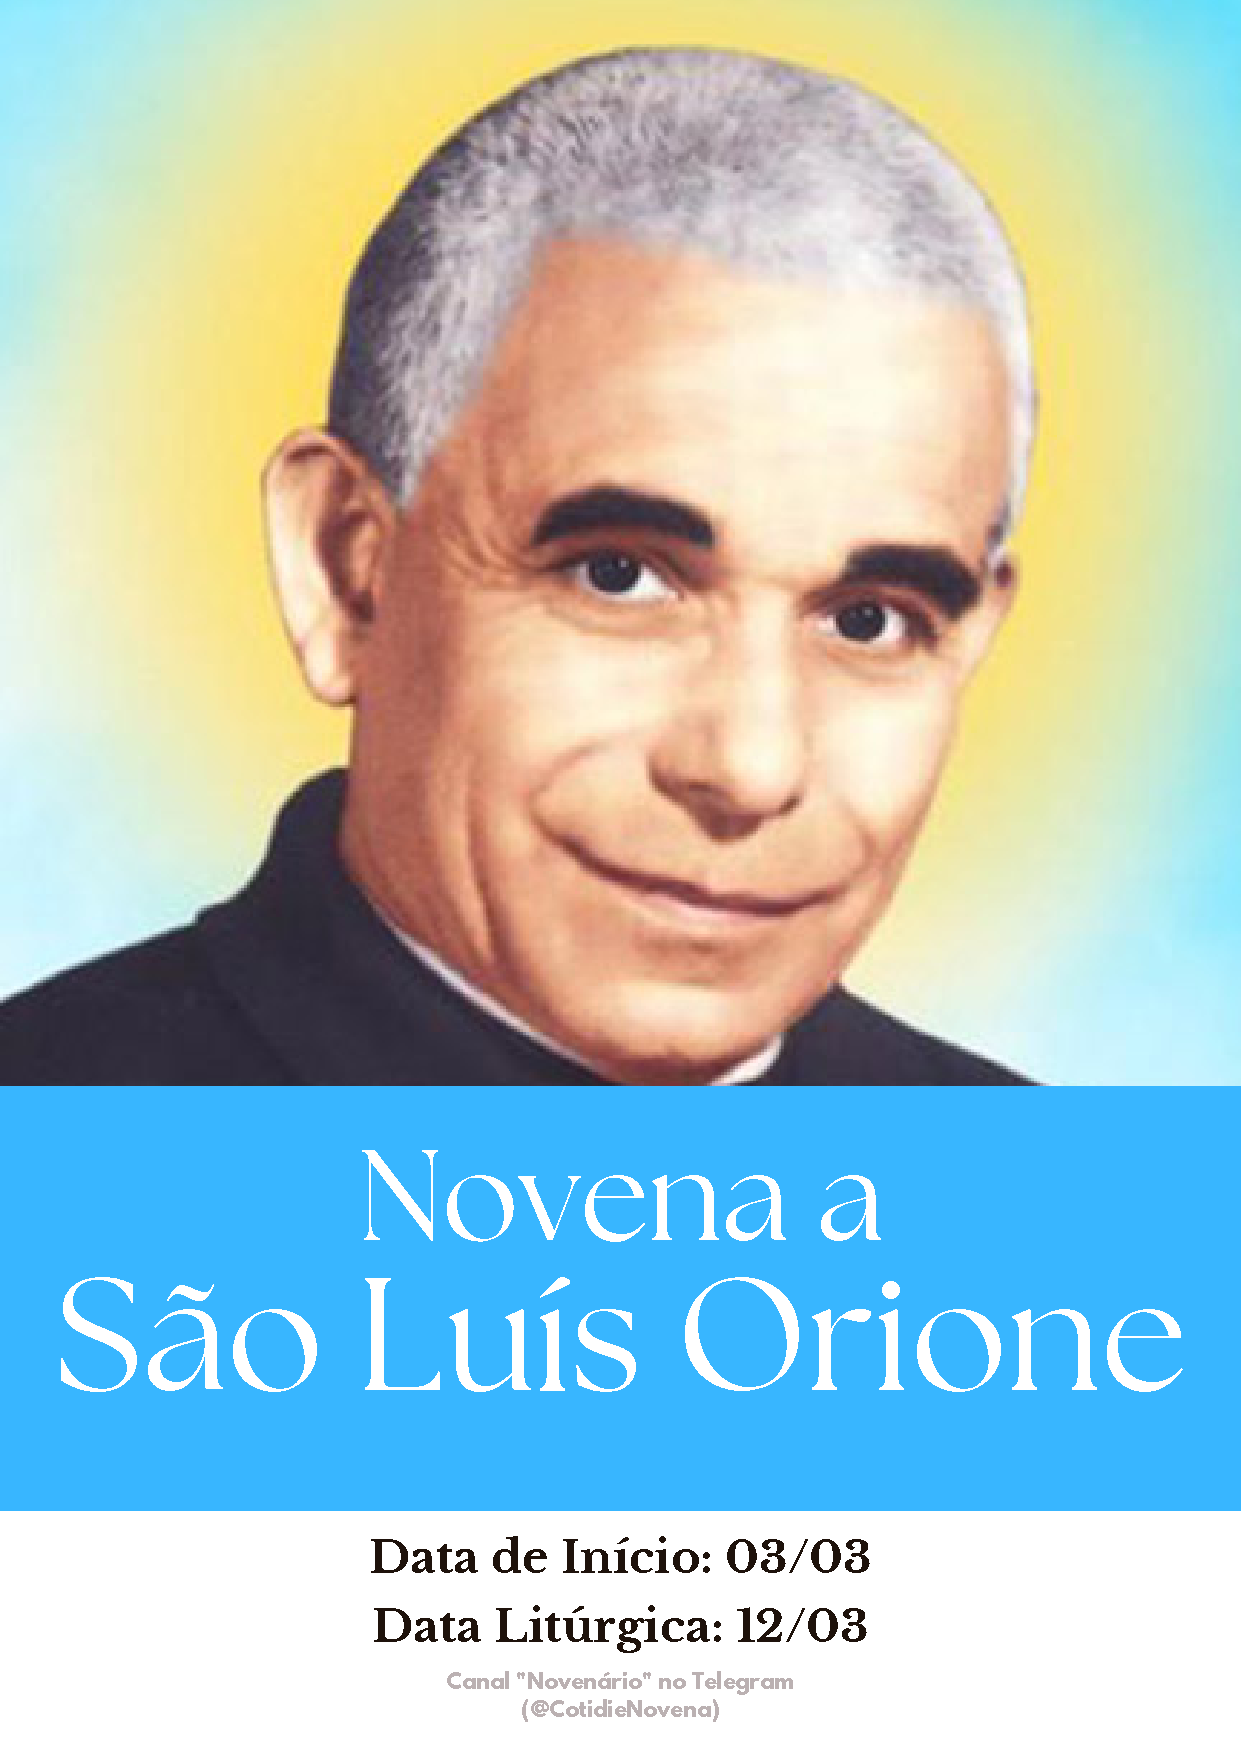
\includepdf[pages=1]{Capa São Luís Orione.pdf}

\begin{center}
  {\huge Novena de São Luís Orione}
\end{center}



\noindent\rule{\textwidth}{0.4pt}

\tableofcontents

\thispagestyle{empty}


% --- Origem ---
\newpage

\section{História}

\subsection{Origens}

Luís Orione nasceu em Pontecuore, Itália, no dia 23 de junho de 1872. Era filho de uma família pobre. Seus pais eram camponeses e muito simples. Porém, sua família era bem estruturada, rica em honestidade e sabedoria. Sua mãe, sábia educadora, serviu de inspiração e modelo por toda a vida. Luis Orione recebeu os fundamentos da sua fé no aconchego de seu lar e isso lhe marcou para o resto a vida.

\subsection{Contato com um santo}

No início da juventude, Luis Orione já pensa em ser sacerdote. Apoiado por sua família, ele ingressou no Oratório Salesiano em Turim, uma obra dedicada à educação e formação de crianças, adolescentes e jovens pobres. O fundador dessa obra era São João Bosco, ou simplesmente Dom Bosco. Este ainda era vivo quando Luís Orione ingressou no Oratório. Dom Bosco tinha grande estima por Orione e percebeu logo a vocação do jovem. Por isso, dedicou especial atenção na formação de Orione.

\subsection{Fundador dinâmico }

Em 1892, sendo ainda seminarista, Luís Orione fundou duas escolas dedicadas à formação de crianças e jovens. Ordenado em 1895, passou, então, a se dedicar aos necessitados com todo ardor e dedicação. Sua meta era acolher e evangelizar os mais necessitados.

\subsection{Missionário da caridade}

O Padre Luís Orione era incansável na sua luta em favor dos necessitados. Por várias vezes empreendeu viagem por toda a Itália pedindo doações e ajuda material para as obras de caridade que ele fundara. Colocava-se como um instrumento nas mãos da Providência Divina, tendo sempre como objetivo o alívio dos sofrimentos e das necessidades humanas.

\subsection{Terremoto}

Em 1908, um terremoto terrível colocou abaixo a região da Sicília e Calábria, na Itália. Luís Orione fez um grande trabalho no socorro das inúmeras vítimas. Tanto que o Papa Pio X pediu que ele ficasse lá por mais tempo. Padre Orione atendeu, ficando lá por três anos.

\subsection{Fundador}

Em 1915, o padre Luís Orione fundou uma congregação que ele chamou de “Pequena Obra da Divina Providência”. O objetivo da obra era atender aos pobres, humildes trabalhadores, doentes, necessitados e, principalmente, aos esquecidos pela sociedade. Posteriormente fundou a Congregação dos Padres Orionitas. Depois, fundou a Congregação das Irmãzinhas Missionárias da Caridade. Mais tarde, fundou a Congregação das Irmãs Sacramentinas. Finalmente, fundou a Congregação dos Eremitas de Santo Alberto. Nessas duas últimas fundações, um dos objetivos era admitir religiosos cegos, coisa que, na época, era difícil. 

\subsection{A obra se estende pelo mundo}

A Congregação dos Filhos da Divina Providência e a das Missionárias da Caridade se expandiram por vários países da Europa. Depois, pelas Américas e pela Ásia. Hoje, a Obra de São Luís Orione tem milhares de Casas e Instituições espalhadas pelo mundo, atuando principalmente na área assistencial e educativa.

\subsection{No Brasil}

A Obra de São Luís Orione está no Brasil desde 1914. São várias casas que abrigam órfãos, excepcionais, deficientes, idosos. Há também hospitais para os necessitados. A obra da Divina Providência sempre foi e ainda hoje continua recebendo toda a manutenção vinda de esmolas e doações. 

\subsection{Morte}

São Luís Orione faleceu como uma vela que se desgastou queimando pelo cansaço missionário. Ele tinha com sessenta e oito anos quando entregou sua alma a Deus, na cidade de San Remo, Itália. Era o dia 12 de Março de 1940. Sua canonização foi celebrada em 2004, pelo Papa João Paulo II, em Roma. São Luís Orione foi um sacerdote humilde e gigante no apostolado da caridade. Foi chamado de pai dos pobres e grande benfeitor da Humanidade aflita e sofredora.

% --- Orações Diárias ---
\newpage

\vfill

\section{Orações}
\subsection{Oração Inicial}\label{sub:inicial} % (fold)

Ó Deus, que fizestes de São Luís Orione um incansável servo dos pobres e um modelo de confiança na Divina Providência, concedei-nos, por sua intercessão, a graça de amar os irmãos com obras e verdade. Que ele, que viveu o Evangelho com radicalidade, nos inspire a ser sinais do Vosso amor no mundo.

Neste momento, apresento a Vós, Senhor, as minhas intenções:
\textit{(coloque aqui suas intenções).}


\subsection{1º Dia - O Chamado à Santidade na Juventude}

\underline{\nameref{sub:inicial}}

São Luís Orione, desde jovem, sentiu o chamado a servir a Deus. Aos 13 anos, entrou no Oratório de São João Bosco, onde aprendeu a amar os jovens e os pobres.
Ó São Luís Orione, que respondeste ao chamado de Deus com generosidade, ajuda-me a discernir minha vocação. Ensina-me a ouvir a voz de Cristo nos pequenos e necessitados. Amém.

\underline{\nameref{sub:final}}


\subsection{2º Dia - A Fundação da Pequena Obra da Divina Providência}

\underline{\nameref{sub:inicial}}

São Luís Orione fundou congregações religiosas, orfanatos e escolas, sempre confiando que "a Divina Providência nunca falta". 

Ó São Luís Orione, que construístes obras de amor com fé inquebrantável, ensina-me a confiar na providência de Deus. Ajuda-me a agir sem medo, sabendo que Ele cuida de tudo. Amém.

\underline{\nameref{sub:final}}


\subsection{3º Dia - O Amor aos Abandonados}

\underline{\nameref{sub:inicial}}

São Luís Orione acolhia órfãos, doentes e pessoas com deficiência, dizendo: "Só a caridade salvará o mundo".
Ó São Luís Orione, que vistes Cristo nos mais frágeis, ajuda-me a enxergar Sua face nos excluídos. Ensina-me a doar meu tempo e recursos aos que sofrem. Amém.

\underline{\nameref{sub:final}}


\subsection{4º Dia - A Devoção à Nossa Senhora}

\underline{\nameref{sub:inicial}}

São Luís Orione tinha uma devoção profunda a Maria, a quem chamava de "Mãe da Divina Providência". Ele via nela o modelo de entrega total a Deus.
Ó São Luís Orione, que amastes a Virgem Maria com ternura filial, ensina-me a recorrer a ela nas dificuldades. Ajuda-me a imitar sua fé e obediência. Amém.

\underline{\nameref{sub:final}}


\subsection{5º Dia - A Coragem nas Adversidades}

\underline{\nameref{sub:inicial}}

São Luís Orione enfrentou perseguições, calúnias e doenças, mas nunca desistiu. Ele dizia: "Avante, sempre avante, e santidade!".
Ó São Luís Orione, que transformastes o sofrimento em oferta a Deus, ajuda-me a aceitar as cruzes com paz. Ensina-me a ver nas provações um caminho de santificação. Amém.

\underline{\nameref{sub:final}}


\subsection{6º Dia - O Zelo Missionário}

\underline{\nameref{sub:inicial}}

São Luís Orione enviou missionários a vários países, pregando que "a Igreja deve ser toda para todos".
Ó São Luís Orione, que sonhavas com uma Igreja servidora, inspira-me a ser missionário onde estou. Ajuda-me a anunciar Cristo com palavras e ações. Amém.

\underline{\nameref{sub:final}}


\subsection{7º Dia - A Humildade no Serviço}

\underline{\nameref{sub:inicial}}

São Luís Orione lavava os pés dos pobres, servia os doentes e comia com os órfãos. Sua humildade era a expressão de seu amor a Cristo.
Ó São Luís Orione, que escolhestes o último lugar para glorificar a Deus, ensina-me a servir sem buscar reconhecimento. Ajuda-me a encontrar alegria na simplicidade. Amém.

\underline{\nameref{sub:final}}


\subsection{8º Dia - A Esperança nas Catástrofes}

\underline{\nameref{sub:inicial}}

São Luís Orione ajudou vítimas de terremotos na Itália, reconstruindo casas e igrejas. Ele acreditava que "depois da noite, vem a aurora".
Ó São Luís Orione, que renovastes a esperança nos desesperados, ajuda-me a confiar na luz de Deus nas trevas. Ensina-me a ser consolo para os que choram. Amém.

\underline{\nameref{sub:final}}


\subsection{9º Dia - O Legado de Amor Eterno}

\underline{\nameref{sub:inicial}}

São Luís Orione partiu para o céu em 1940, deixando um legado de obras de caridade que continuam até hoje. Ele dizia: "Morreremos, mas a Obra de Deus não morrerá".
Ó São Luís Orione, que entrastes na glória dos santos, intercedei para que eu viva uma morte santa. Concede-me a graça de deixar um rastro de amor no mundo. Amém.

\underline{\nameref{sub:final}}

\subsection{Oração Final}\label{sub:final} % (fold) \subsection{Orações de Cada Dia}

\[\textbf{Pai-Nosso, Ave-Maria, Glória}\]

Ó Deus, que fizestes de São Luís Orione um apóstolo da caridade e pai dos pobres, concedei-nos, por sua intercessão, a graça de imitar seu amor concreto aos necessitados. Que ele, que confiou na Divina Providência até o fim, nos ensine a servir com fé e alegria.

Lembrai-Vos, Senhor, das minhas intenções e concedei-me as graças que Vos peço, para a Vossa glória e o bem da minha alma. Por Cristo, Nosso Senhor. Amém.


\vfill

\begin{center}
\subsection*{Fontes:}
Adaptado de: {\color{blue} \underline{\href{https://cruzterrasanta.com.br/historia-de-sao-luis-orione/362/102/}{Cruz Terra Santa}}} e {\color{blue} \underline{\href{https://youtube.com/playlist?list=PLN7jQwkJvdQoCTF1o4mfX_l-SMaw4goe0&si=srrIsdAAgNtQvnvw}{Canal A Oração dos Santos}}}
\end{center}


\end{document}
